\chapter{Interpolation des données d'une base}
  \section{Généralités}\label{general}
    L'utilisation de l'\ipp s'effectue de la même façon que les autres méthodes d'\EOS,
    la déclaration se fait à l'aide de la méthode \str{\IPP}
    et d'une référence correspondant au nom du fichier au format ``med'', contenant la \bdd, exemple:
    \vspace{0.3cm}
    \begin{itemize}
     \item[\ding{0}] \Cpp{\EOS\ obj\_ipp(\str{\IPP}, \str{med\_file});}
    \end{itemize}
    \vspace{0.5cm}
    
    Avec ce constructeur toutes les propriétés de la \bdd\ sont chargées.
    \smallbreak
    \vspace{0.2cm}
    A noter, il est possible de faire un chargement sélectif, en spécifiant une liste de propriétés à l'instanciation de l'objet \EOS: 
    
    \vspace{0.3cm}
    \begin{itemize}
      \item[\ding{0}] \Cpp{Strings list(3);}
      \item[\ding{0}] \Cpp{list[0] = \str{T\_sat};}
      \item[\ding{0}] \Cpp{list[1] = \str{rho};}
      \item[\ding{0}] \Cpp{list[2] = \str{Cp};}
      \item[\ding{0}] \Cpp{\EOS ipp(\str{\IPP},\str{med\_file},list);}
    \end{itemize}
    \vspace{0.5cm}
     
    Le module de l'\ipp\ contient une classe principale \IPP\ ainsi que 2 classes dérivées, une pour la phase liquide et une pour la phase vapeur,
    respectivement: \IPPl\  et \IPPv. Ces 2 classes filles contiennent une surcharge des fonctions ``compute'' dans le plan \textbf{pT}.


    \section{Chargement des données de la classe \IPP}
       
    \subsection{Entête}
    L'entête du fichier med (\Cpp{header}), permet notemment au 
    programme de récupérer le couple méthode/référence, utilisé pour créer la \bdd.
    Ces valeurs sont, ensuite, affectées sous forme de chaînes de caractères, aux attributs \Cpp{base\_method} et \Cpp{base\_reference}.
    
    \subsection{Maillages}\label{maillages}
    Les maillages enregistrés dans la \bdd\ possèdent les dénominations suivantes:
    \vspace{0.3cm}
    \begin{itemize}
      \item[\ding{192}] \pph: \str{ph\_domain};
      \item[\ding{193}] saturation: \str{sat\_domain} (\sgp);
      \item[\ding{194}] spinodal: \str{lim\_domain} (\sgp).
    \end{itemize}
    \vspace{0.5cm}
    
    Cet aiguillage permet l'affectation des attributs, respectif à chaque maillage:
    \vspace{0.3cm}
    \begin{itemize}
      \item Valeurs des noeuds: \Cpp{n\_p\_ph} \ding{192}, \Cpp{n\_h\_ph} \ding{192}, \Cpp{n\_p\_satlim} \ding{193}\ding{194};
      \item Domaine d'étude: \Cpp{nodes\_ph} \ding{192}, \Cpp{nodes\_sat} \ding{193}, \Cpp{nodes\_lim} \ding{194};
      \item Vecteur de connectique (Cf. paragraphe \ref{connectique}):
      connect\_ph \ding{192}, connect\_sat \ding{193}, connect\_lim \ding{194};
      \item Numérotation des cellules: index\_conn\_ph \ding{192}.
    \end{itemize}
    \vspace{0.5cm}
    
    \subsection{données scalaires}
    Les données scalaires décrivant les maillages de la \bdd\ sont affectées aux attributs suivants:
    \vspace{0.3cm}
    \begin{itemize}
      \item \Cpp{pmin}: Pression minimum
      \item \Cpp{pmax}: Pression maximum
      \item \Cpp{hmin}: Enthalpie minimum
      \item \Cpp{hmax}: Enthalpie maximum
      \item \Cpp{tmin}: Température minimum
      \item \Cpp{tmax}: Température maximum
      \item \Cpp{delta\_p\_f}: Ecart en pression de la maille la plus raffinée\footnote{Taille en pression ou en enthalpie 
      d'une maille du maillage global Cf. paragraphe \ref{raflocal}\label{delta}}
      \item \Cpp{delta\_h\_f}: Ecart en enthalpie de la maille la plus raffinée\textsuperscript{ \ref{delta}}
      \item \Cpp{tcrit}: Température critique du fluide
      \item \Cpp{pcrit}: Pression critique du fluide
      \item \Cpp{hcrit}: Enthalpie critique du fluide
    \end{itemize}
    \vspace{0.5cm}
    
    \subsection{propriétés}
    L'\ipp charge les valeurs des propriétés de la \bdd\ med en mémoire,
    soit dans son integralité soit par sélection définie par l'utilisateur (Cf. Paragraphe \ref{general}).
    \smallbreak\vspace{0.3cm}
    Toutes les valeurs, des propriétés chargées, aux \n s des maillages
    sont stockées dans le tableau \Cpp{all\_prop\_val}\footnote{La nécessité de stocker les tableaux
    de valeurs compris dans les champs, vient du choix de développement qu'à la création d'un objet de la classe \FIELD,
    ce tableau doit lui être passé par référence.\label{field}}.
    Par contre les champs des propriétés sont affectées avec la distinction du maillage sur lequel ils s'appliquent 
    (Cf. paragraphe \ref{maillages}). Il y a donc 3 attributs à la classe \IPP\ comprenant ces champs:
    \vspace{0.3cm}
    \begin{itemize}
      \item \Cpp{val\_prop\_ph} \ding{192}
      \item \Cpp{val\_prop\_sat} \ding{193}
      \item \Cpp{val\_prop\_lim} \ding{194}
    \end{itemize}
    \vspace{0.5cm}
    
    \subsection{Erreurs}
    Les erreurs, considérés ici, proviennent de la méthode avec laquelle a été créée la \bdd.
    Elles sont stockées sous forme d'un tableau, par propriété, qui contient l'erreur à chaque \n\ du maillage.
    Cependant, lors du chargement, un traitement est effectué pour que l'erreur soit étendu à la maille,
    car si un des \n s de la maille est faux alors toutes les valeurs interpolées dans cette maille sont en erreur.
    \smallbreak\vspace{0.3cm}
    De la même façon que pour les propriétés il y a 1 attribut qui stocke tous les tableaux des erreurs 
    relevées\footnote{Même fonctionnement de la classe \EFIELD\ que la classe \FIELD, voir note \ref{field}} (\Cpp{all\_err\_val})
    et 3 attributs déffinissant les champs d'erreurs dans les maillages:
    \vspace{0.3cm}
    \begin{itemize}
      \item \Cpp{err\_cell\_ph} \ding{192}
      \item \Cpp{err\_segm\_sat} \ding{193}
      \item \Cpp{err\_segm\_lim} \ding{194}
    \end{itemize}
    \vspace{0.5cm}
   
   
   \section{Connectique}\label{connectique}
   
   Etant donné l'irrégularité des tailles de mailles, due au raffinement local, le repérage d'un point dans un maillage, est réalisé à partir
   de la succession de vecteurs d'indices d'équivalence,
   d'un repère à un autre, c'est ce qui est appelé connectique. Elle assure, lors d'un calcul d'une propriété en un point quelconque du maillage, 
   que l'interpolation est réalisée avec les points rééls ou de continuité les plus proches.
   \vspace{0.3cm}
   \begin{itemize}
     \item[\textbullet] \textbf{Le positionnement d'un point sur le \sgp:}\\
     Le positionnement d'une valeur en pression ($p$), est réalisé en récupérant le premier indice ($i$) des vecteurs
     \Cpp{connect\_sat} ou \Cpp{connect\_lim}, pour lequel la valeur \Cpp{nodes\_sat} ou \Cpp{nodes\_lim} respectivement, est supérieure à $p$.
     Les indices des valeurs de \Cpp{nodes\_sat} ou \Cpp{nodes\_lim}, sont donc $i-1$ et $i$.
%      \smallbreak\vspace{0.3cm}
%      L'intérêt de passer, ici, par un vecteur de
%      connectique intermédiaire reste à determiner.
     \smallbreak\vspace{0.3cm}
     \item[\textbullet] \textbf{Le positionnement d'un point dans le \pph:}\\
      Lors du chargement des données, l'attribut vecteur \Cpp{fnodes2phnodes}, de la classe \IPP,
      est affecté pour chaque maille du maillage global (mailles fictives, Cf. Paragraphe \ref{raflocal})
      par l'indice du premier \n\ de cette maille (plus petites valeurs de \textbf{p} et de \textbf{h}).
      \smallbreak\vspace{0.3cm}
      Lors du calcul d'une propriété en un point $i$,
      le point est positionné, dans un premier temps, dans la maille fictive ($m$),
      à l'aide des données \Cpp{delta\_p\_f} et \Cpp{delta\_h\_f}. 
      Puis dans un second temps l'indice du premier \n\ de $m$ est récupéré, avec \Cpp{i=fnodes2phnodes[m]}.
      Enfin les indices des 4 \n s de la maille encadrant le point, correspondent aux valeurs comprises dans l'intervalle:
      \begin{align*}
      [connect\_ph[i];connect\_ph[i+3]];
      \end{align*}
      Avec, \Cpp{connect\_ph[i]} vecteur de correspondance \n s~fictifs/\n s~réels.
      \smallbreak\vspace{0.3cm}
   
   \end{itemize}
   \vspace{0.5cm}
   
   
   \section{Interpolation}
   
    \subsection{Calculs des propriétés}
    
    Selon la propriété calculée, les grandeurs peuvent être interpolées directement ou déduites:
    
    \subsubsection{Grandeurs interpolées directement}
    \begin{itemize}
      \item La température de saturation (\textbf{T\_sat});
      \item Toutes les dérivées par rapport à \textbf{p};
      \item Les enthalpies dans le domaine spinodal et dans le plan \textbf{pT} \textbf{(h\_l\_lim}, \textbf{h\_v\_lim}, \textbf{h\_pT});
      \item Toutes les propriétés du \pph;
      \item Toutes les dérivées des propriétés du \pph.
    \end{itemize}
    A noter, qu'aucune cohérence n'est faite dans l'interpolateur, entre les grandeurs et leurs dérivées.
    
    \subsubsection{Grandeurs déduites}
    \begin{itemize}
      \item Toutes les propriétés dans le plan \textbf{pT}, en dehors de \textbf{h\_pT};
      \subitem Le calcul dans le plan \textbf{pT}, par exemple pour la propriété \textbf{rho}, passe par l'intermédiaire suivant:
      \begin{align*}
      &rho(p,T) = rho(p,h)\\
      &\text{Avec, } h = h(p,T)\\
      &=> T = T(p,h)
      \end{align*}
      
      \item Toutes propriétés dans le domaine de saturation, en dehors des dérivées et de \textbf{T\_sat}.
      \subitem Le calcul des grandeurs à saturation passe par plusieurs calculs intermédiaires, par exemple pour propriété \textbf{rho\_l\_sat}:\\
       \begin{align*}
	&rho^l_{sat}(p) = rho(p,h^l_{sat})\\
	&\text{Avec, } h^l_{sat} = h^l(p,T_{sat})\\
	&=> T_{sat} = T(p,h^l_{sat}) = T(p,h^v_{sat})
       \end{align*}
    \end{itemize}
    A noter, les grandeurs détuites assurent la cohérence entre les propriétés du \pph\ et les grandeurs de saturation.

    \subsection{Interpolation}
    \begin{itemize}
      \item[\textbullet] L'interpolation des valeurs sur le \sgp\ se fait de façon linéaire.
      \item[\textbullet] Dans le \pph\ l'interpolation est dite ``bilinéaire'':
       \smallbreak\vspace{0.3cm}
       L'exemple qui suit, présente le calcul de la valeur d'une proriété $f$ au point $i$, de coordonnées ($h_i$,$p_i$). 
       Le point $i$ est situé dans une maille comprenant les 4 \n s a, b, c et d (Cf Figure \ref{schinter}).
       \begin{figure}[H]
	 \center
	 \includegraphics[width=0.4\textwidth]{schema_inter.eps}
	 \caption{Interpolation au point $i$ dans une maille du \pph.}\label{schinter}
       \end{figure}
       
       Par interpolation bilinéaire l'expression de $f$ au point $i$ s'écrit:
       
       \begin{align}
       \label{intereq}
       f_i &=  f_a\cdot(1 - \Delta_p - \Delta_h + \Delta_p\cdot\Delta_h)\\
           &+ f_b\cdot(\Delta_h -  \Delta_p\cdot\Delta_h)\nonumber\\
	   &+ f_c\cdot(\Delta_p\cdot\Delta_h)\nonumber\\
	   &+ f_d\cdot(\Delta_p - \Delta_p\cdot\Delta_h)\nonumber
       \end{align}
       


       Avec,\\
      \begin{minipage}{0.49\linewidth}
      \begin{align}
	\label{deltp}
	\Delta_p = \frac{p_i - p_a}{p_d - p_a}
      \end{align}
      \end{minipage}
      \begin{minipage}{0.49\linewidth}
      \begin{align}
	\label{delth}
	\Delta_h = \frac{h_i - h_a}{h_b - p_a}
      \end{align}
      \end{minipage}

      \vspace{0.5cm}
      \item[\textbullet] Dans le plan \textbf{pT} l'inversion h(p,T) est réalisée:
      \smallbreak\vspace{0.3cm}
      En utilisant le schéma de la figure \ref{schinter}, pour déterminer $h_i$ à $p_i$ et $T_i$ donnés.
      \smallbreak\vspace{0.2cm}
      Dans toutes les mailles réelles, les étapes suivantes sont effectuées:
      \begin{itemize}
	\item Récupération des valeurs de $p$ , $h$ et $T$ aux 4 \n s a, b, c et d 
	\item verification si $p_a < p_i < p_d$\\
	Si vrai:
	\item à partir de l'équation \ref{intereq}, $\Delta_h$ est determiné: 
	\begin{equation}
	  \label{delheq}
	  \Delta_h = \frac{T_i + \Delta_p\cdot(T_a - T_d) - T_a}{T_b - T_a + \Delta_p\cdot(T_a + T_c - T_d - T_b)}
	\end{equation}
	L'équation \ref{delth} induit: 
	\begin{equation}
	h_i = \Delta_h\cdot(h_b - h_a) + h_a
	\end{equation}	
      \end{itemize}
      La méthode est peu optimisée, dans le mesure où, toutes les mailles sont chargées. 
      De plus il y a interpolation pour toutes celles qui respectent: $p_a < p_i < p_d$.
      
      
    \end{itemize}
    
   
    
 
  
  
  \clearpage
      

\clearpage

